\documentclass{beamer}
\usetheme{Goettingen}
% \usetheme[uttitlepage=false]{ut}
% \usetheme[euler=false,titlepagebg=B]{ut}
% \usetheme[titlepage=C,debug]{ut}
% \usetheme[titlepage=A]{ut}


\title[Growth Models]{The Growth Models for Science of Cities}
% \subtitle[Short subtitle]{I am not using any subtitles}
\author[G. Xiu]{Gezhi Xiu} %  
\institute[IRSGIS PKU]{Complexity Research Group,\\Peking University}
\date[\today]{\today}

\begin{document}


\maketitle
\begin{frame} \frametitle{Contents}
\tableofcontents
\end{frame}
\section{Overview}
\begin{frame}{Overview}
  \begin{itemize}
    \item Zipf's law and its formation
    \begin{itemize}
      \item Zipf's law without fine-tuning: static mesoscopic
      \item Stationary distribution of dynamical processes for the sizes of groups of individuals
      \begin{itemize}
        \item mesoscopic: cities
        \item microscopic: individuals
      \end{itemize}
    \end{itemize}
    \item Gibrat's law and Taylor's law
  \end{itemize}
\end{frame}

\section{Existing Models}

\subsection{Fractal Cities}

\begin{frame}{Fractal Cities}
  \begin{itemize}
    \item M. Batty and P. Longley, Fractal Cities: A Geometry of Form
    and Function (Academic, San Diego/London, 1994).
    \item Cellular automata have been used to model spatial structure of urban land use over time: Environ. Plan. A 25, 1175 (1993).
    \item The correlated percolation model
    
  \end{itemize}
\end{frame}

\subsection{Zipf's law}
\begin{frame}{Zipf's law}
  The group size distribution.
  \begin{itemize}
    \item the number of employees in firms
    \item the distribution of family names
    \item the distribution of city sizes
    
  \end{itemize}

  \begin{align}
    P(n)&\sim n^{-1-\gamma}\\
    \gamma&\simeq 1
  \end{align}
  
\end{frame}

\begin{frame}{Models that lead to Zipf's law}
Some up-to-date models are really fascinating.
  \begin{itemize}
    \item Models with latent variables can lead to Zipf's law without fine-tuning by mixing together narrow distributions with very different means.(PRL 113, 068102 (2014))
    \begin{itemize}
      \item static systems (no time dependence)
    \end{itemize}
    \item The stationary distribution of dynamical processes for the sizes of groups of individuals
    \begin{itemize}
      \item mesoscopic models at the scale of the groups (e.g., cities) Am. J. Phys. 58, 267 (1990). Variance that is not Gaussian but exponential Gaussian leads to Zipf's law.
      \item microscopic models at the scale of the individuals (e.g., dwellers)
    \end{itemize}
  \end{itemize}
  
\end{frame}

\begin{frame}{Mesoscopic Models}
\begin{itemize}
  \item without the need to fine-tune their parameters to specific values
  \begin{itemize}
    \item random multiplicative process, Am. J. Phys. 58, 267 (1990).\emph{space independent}
    \item Gibrat's law / proportionate random growth, Phys. Rev. E 57, 4811 (1998).
    \item the interplay between intermittency and diffusion, Phys. Rev. E 58, 295 (1998).
  \end{itemize}
  \item however they are coarse-grained descriptions of population dynamics and lack an explicit link to the underlying microscopic processes
\end{itemize}  
\end{frame}

\begin{frame}{Microscopic Models}
  \begin{itemize}
    \item Stochastic processes describing the events experienced by an individual, namely births, deaths, and migrations, that ultimately determine the change in the size of a population.
    \begin{itemize}
      \item Yule's and Simon's models: rich-get-richer, Phil. Trans. R. Soc. Lond. B 213, 21 (1925), Biometrika 42, 425 (1955).
      \item Cluster growth and aggregation, Phys. Rev. E 58, 7054 (1998). 
      \item Reaction diffusion models: explore the role of intermittency in creating spatial inhomogeneities in agreement with Zipf’s law, Phys. Rev. Lett. 79, 523
      \item Preferential migration to large aggregates, Phys. Rev. Lett. 88, 068301 (2002).
      \item Spatial explicit preferential attachment: the probability that a city grows is essentially assumed to be proportional to the size of the city.
      \item network growth with redirection, Phys. Rev. X 4, 011008 (2014).
    \end{itemize}
    \item Only for fine-tuned parameters to get $\gamma=1$.
  \end{itemize}
\end{frame}

\subsection{Radical Decay}
\begin{frame}{Radical Decay}
  \begin{itemize}
    \item The correlated percolation model: an urban built environment is shaped by spatial correlations where the occupation probabilities of two sites are more similar the closer they are.
  \end{itemize}
\end{frame}

  %% Taylor's law
\subsection{Taylor's law}

  \begin{frame}{Taylor's law}
    \begin{figure}
      \centering
      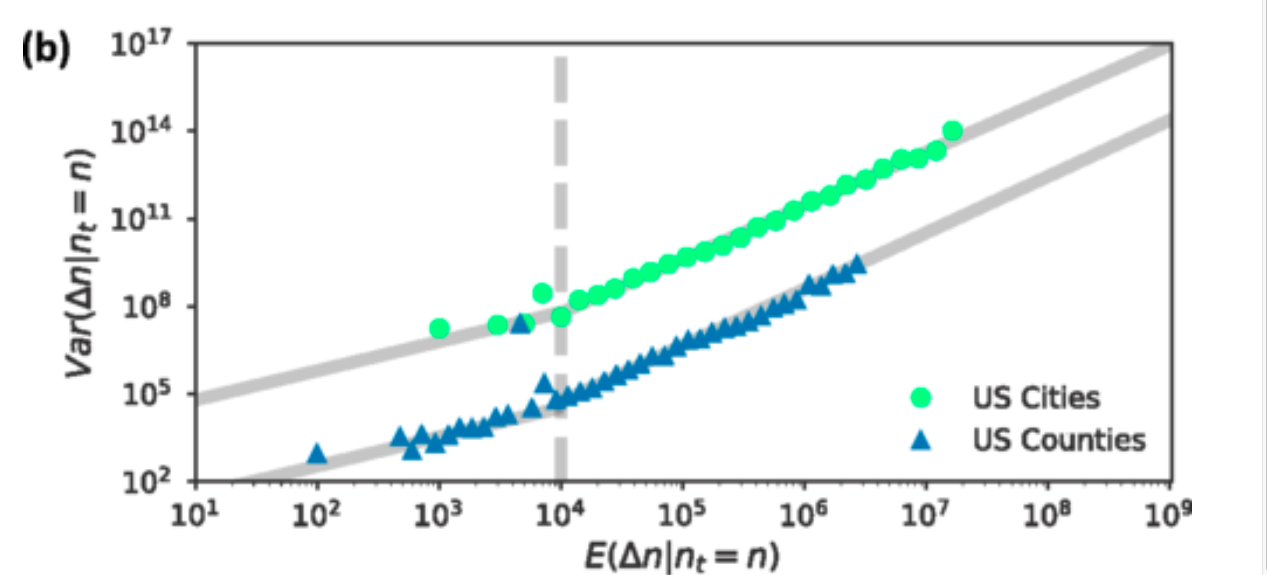
\includegraphics[width = 0.5\linewidth]{pics/taylor's.png}
      \caption{The variance of population in year $t+1$ conditioned to the population in year $t$ ($y$ axis) vs the average population in year $t+1$ conditioned to the population in year $t\ (x$
       axis) for cities (circles) and counties (triangles) in the United States during the period 1970–2010.}
    \end{figure}
  \end{frame}


\section{Spatial Yule Models}

\begin{frame}{My Current Work: Spatial Yule Model}
  How can we address more aspects of urban studies within a simpler model?
\end{frame}

\begin{frame}{Observations}
  \begin{figure}
    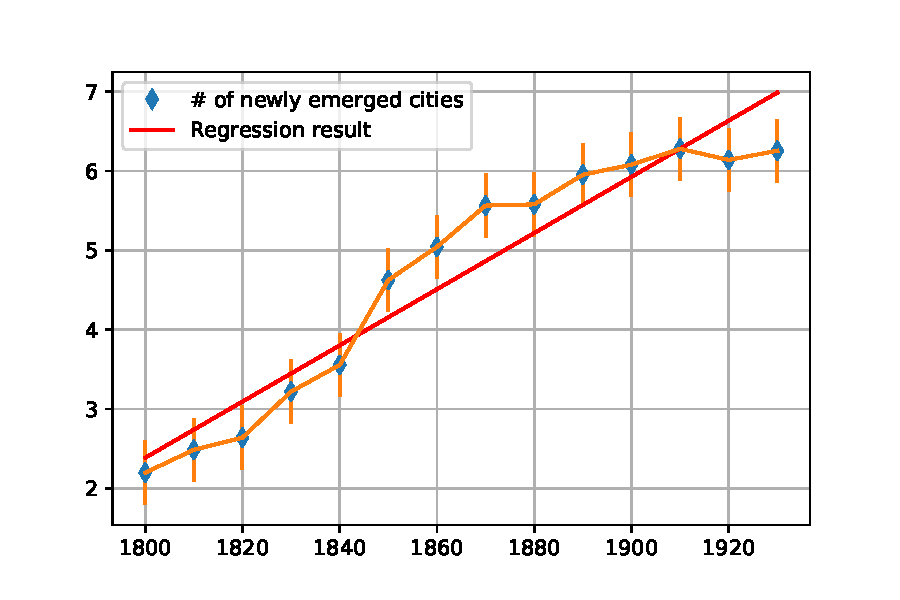
\includegraphics[width=0.48\linewidth]{pics/city_emerge.pdf}
    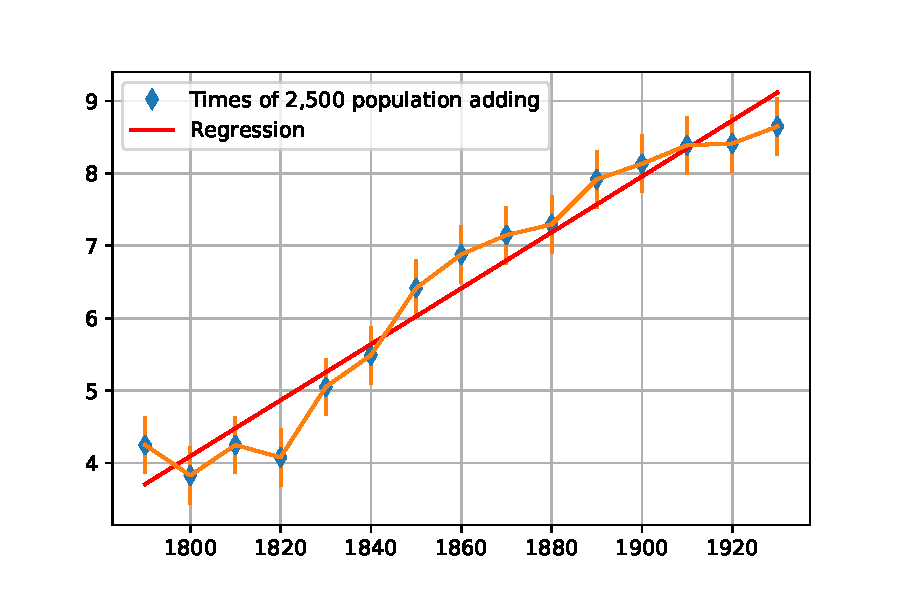
\includegraphics[width=0.48\linewidth]{pics/metapop_adding.pdf}
    \caption{We take 2,500 as the study unit and get a) The emerging speed of cities in the United States, and b) the counts that 2,500 population are added to an existing city. Both slopes are around 0.04, $p<0.0001$.}
  \end{figure}
\end{frame}

\begin{frame}{Population based spreading}
  \begin{figure}
    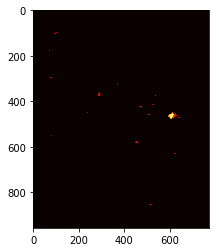
\includegraphics[width = 0.34\linewidth]{pics/ntl/ntl_4.png}
    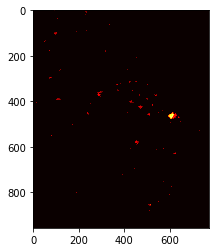
\includegraphics[width = 0.34\linewidth]{pics/ntl/ntl_3.png}
    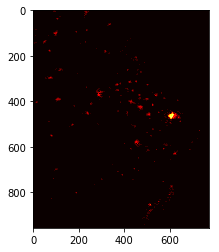
\includegraphics[width = 0.34\linewidth]{pics/ntl/ntl_2.png}
    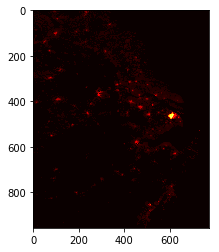
\includegraphics[width = 0.34\linewidth]{pics/ntl/ntl_1.png}
  \end{figure}
\end{frame}

\begin{frame}{Population based spreading}
  \begin{figure}
    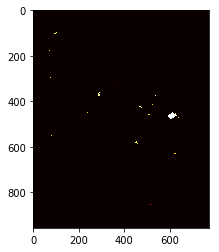
\includegraphics[width = 0.34\linewidth]{pics/ntl/jzh/jzh4.png}
    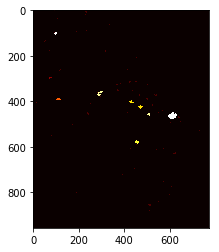
\includegraphics[width = 0.34\linewidth]{pics/ntl/jzh/jzh3.png}
    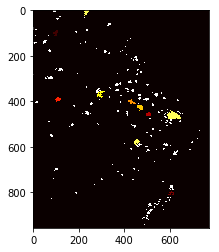
\includegraphics[width = 0.34\linewidth]{pics/ntl/jzh/jzh2.png}
    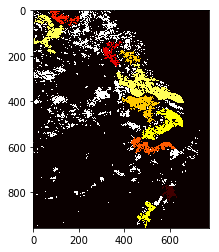
\includegraphics[width = 0.34\linewidth]{pics/ntl/jzh/jzh1.png}
  \end{figure}
\end{frame}

\subsection{Formation Philosophy}
\begin{frame}{Formation Philosophy}
  \begin{itemize}
    \item Scaling of inner- intra-city (area, population, infrastructure)
    \begin{itemize}
      \item Gradient descent to the sum of two-dimensional normal distributions for a optimal locating problem lead to some scaling behavior.
    \end{itemize}
    \item Interacting cities lead to Zipf's law and fractality of urban boundary. 
    \item Asymptotic behaviors (standard cause of scaling) is far from reality.
  \end{itemize}
\end{frame}

\begin{frame}{Rules}
  The background is on a $L\times L$ grid space. The growing mechanism states as follows:
  \begin{enumerate}
    \item Growth rate per capita $\beta_2$, and the growth rate for \# of cities $\beta_1$. 
    \begin{itemize}
      \item ignoring the correspondence to real-life time scale, the actual effective parameter the relative $\beta:=\beta_2/\beta_1$.
    \end{itemize}
    \item The distance a ball lands a meta-population nearby as a constant, $r$, towards a random direction $\theta$. 
    \item The \emph{productive} balls are limited, with no more than $N^*$. 
  \end{enumerate}
\end{frame}

\begin{frame}{Points}
  \begin{enumerate}
    \item possessiveness
    \item homogeneity
    \item cut-off
    \begin{itemize}
    \item comparing to logistic?
    \end{itemize}
  \end{enumerate}
  \vspace{1cm}
  \begin{itemize}
    \item The settings provide a border line between free growth (Scaling laws) and constrained growth (vicissitude phenomena).
  \end{itemize}
  
\end{frame}

\subsection{Results}
\begin{frame}{Results}
  \begin{itemize}
    \item Clark's law of urban population density
    \item Zipf's law of city population sizes
    \item vicissitude
    \item fractality
  \end{itemize}
\end{frame}

\begin{frame}{Clark's law}
  \begin{figure}
    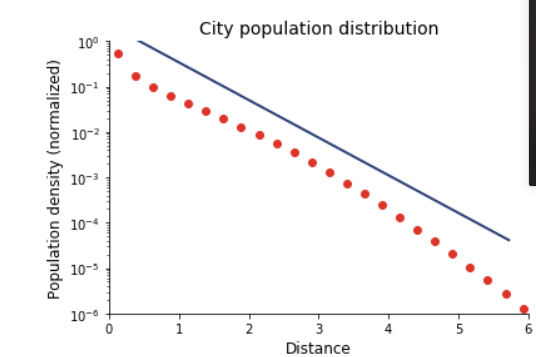
\includegraphics[width = 0.8\linewidth]{pics/clark.PNG}
    \caption{The popualtion density as a function of distance from urban center.}
  \end{figure}
\end{frame}

\begin{frame}{Zipf's law}
  \begin{figure}
    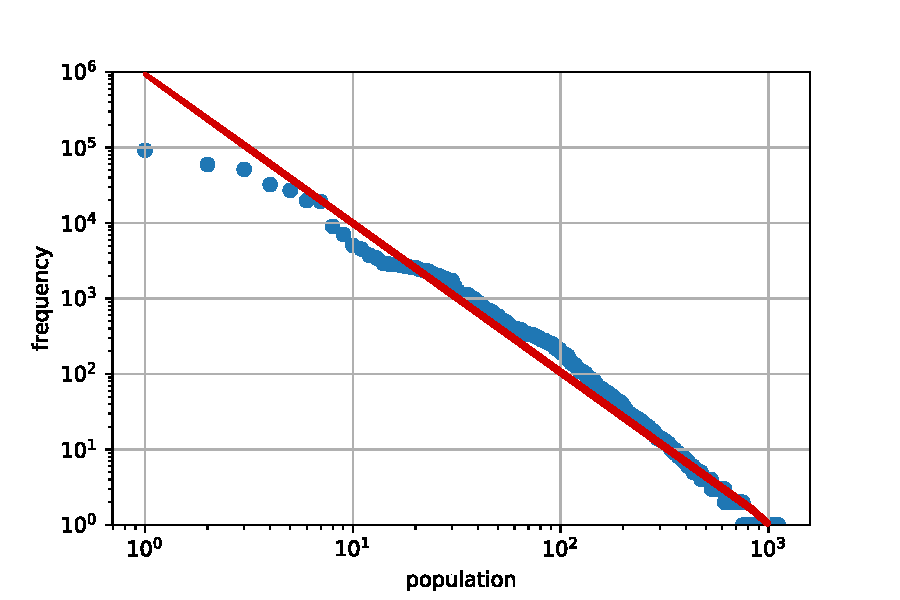
\includegraphics[width = 0.8\linewidth]{pics/zipf.pdf}
  \end{figure}
  $$P(n)\sim n^{-2}$$
\end{frame}

\begin{frame}{Scaling}
  \begin{figure}
    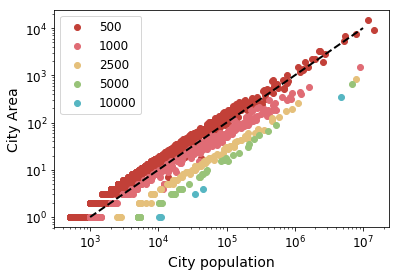
\includegraphics[width = 0.8\linewidth]{pics/pop-area.png}
    \caption{Population versus area}
  \end{figure}
\end{frame}

\begin{frame}{Vicissitude}
  \begin{itemize}
    \item Blockwise
  \begin{align}\rho_{threshold} = k\beta_1/(2\beta_2)+N^*/2\end{align}
    \item Citywise
    \begin{figure}
      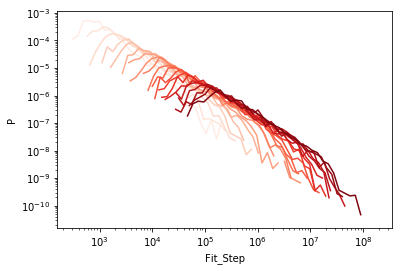
\includegraphics[width = 0.8\linewidth]{pics/step_number.png}
    \end{figure}
  \end{itemize}
\end{frame}

\begin{frame}{Fractality}
  \begin{figure}
    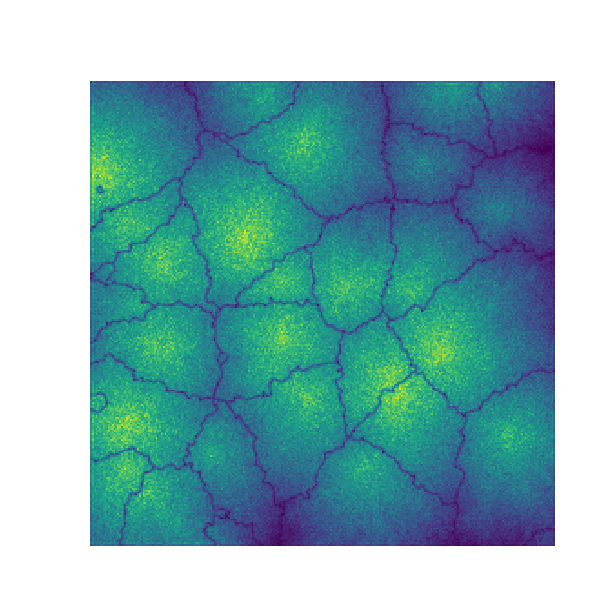
\includegraphics[width = 0.7\linewidth]{pics/fractal_41_256.pdf}
    \caption{Fractality is driven by the probabilistic competition for edging space.}
  \end{figure}
\end{frame}

\begin{frame}{Topics about \emph{what is a city}?}
  Owuor Otieno, Mark . (2017, October 23). What is the Difference Between a City and a Town? Retrieved from https://www.worldatlas.com/articles/what-is-the-difference-between-a-city-and-a-town.html
\end{frame}

\end{document}